\section{Sincronizzazione}
Nei capitoli precedenti abbiamo visto come avviene la comunicazione tra diversi processi, tuttavia, anche se questa gioca un ruolo importante nei sistemi distribuiti non è tutto. Strettamente correlato alla comunicazione è il modo in cui i processi cooperano tra loro e si sincronizzano.\\
La cooperazione è ottenuta parzialmente tramite il naming che permette ai processi di condividere le risorse o comunque le entità.
In questo capitolo ci concentreremo su come i processi possono sincronizzarsi . Partiremo dalla sincronizzazione basata sul tempo reale per poi proseguire con la sincronizzazione in cui conta solo l'ordine relativo. Infine analizzeremo come un gruppo di processi possa eleggere un coordinatore per mezzo di algoritmi di elezione.
\subsection{Sincronizzazione nei sistemi distribuiti}
Il problema della sincronizzazione si presenta anche nei sistemi non distribuiti, tuttavia la distribuzione complica molto le cose in quanto vi sono alcune caratteristiche che nei sistemi centralizzati o monoprocessore non si presentano come:
\begin{itemize}
\item L'assenza di un clock fisico globale.
\item L'assenza di un area di memoria condivisa.
\item La possibilità di avere dei fallimenti parziali
\end{itemize}
In un sistema centralizzato il tempo non è ambiguo, quando un processo vuole conoscere data e ora attuali esegue una chiamata di sistema e il kernel glie la indica. Se un processo $A$ richiede la data e l'ora e un processo $B$ la richiede poco dopo il valore che $B$ otterrà sarà leggermente superiore di quello del processo $A$. In un sistema distribuito invece non è semplice mantenere un'ora e una data comuni a tutte le macchine.\\
Come esempio prendiamo le implicazioni di un orario globale per la funzione \emph{make} di UNIX. Di solito i programmi molto grandi sono divisi in più file sorgenti, per non dover ogni volta compilare tutti i file il \emph{make} esamina la data e l'ora dell'ultima modifica del file sorgente e di quello oggetto. Se il file sorgente \emph{input.c} è stato modificato all'istante 2051 mentre il file oggetto \emph{input.o} è stato modificato all'istante 2050 il \emph{make} sa che il file sorgente è stato modificato e lo deve quindi ricompilare.\\
Supponiamo ora di spostarci in un sistema distribuito in cui non ci siano una data ed un'ora globali. Supponiamo che il file \emph{output.o} abbia associato l'istante 2144; il file \emph{output.c} viene modificato su una macchina diversa che ha il clock leggermente in ritardo rispetto a quella dove risiede \emph{output.o} e perciò gli viene assegnato l'istante 2143 come mostrato in \figurename\,\ref{fig:maketime}.
\begin{figure}
\centering
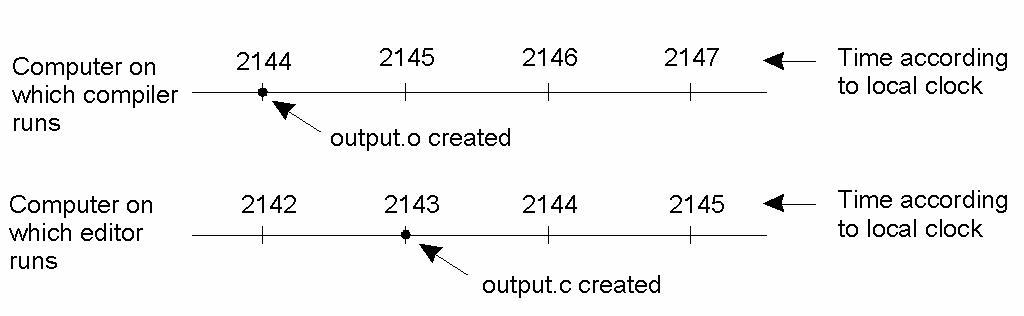
\includegraphics[scale=0.5]{img/maketime.png}
\caption{Assegnamento di istanti di modifica su due macchine diverse}\label{fig:maketime}
\end{figure}
Se ora eseguiamo il \emph{make} esso non richiamerà il compilatore in quanto l'istante di modifica del file sorgente e precedente a quello del file oggetto procurando notevoli problemi al programmatore.
\subsubsection{Orologi fisici}
Praticamente tutti i computer hanno un circuito per tener traccia del tempo; nonostante l'ampio uso che si fa della parola "clock" per indicare questi dispositivi non si tratta realmente di orologi ma si tratta più di \textbf{timer}.
Tale timer di solito è un cristallo di quarzo che oscilla a una frequenza ben definita se sottoposto a tensione, che dipende dal tipo di cristallo, da come è tagliato e dal livello di tensione applicato. Ad ogni cristallo inoltre sono associati un \textbf{contatore} \emph{(counter)} ed un \textbf{registro di mantenimento} (\emph{holding register}). Ogni oscillazione del cristallo decrementa il contatore di uno. Quando il contatore raggiunge lo zero viene generato un interrupt e il contatore viene resettato con il valore contenuto nell'holding register. Ogni interrupt è chiamato \textbf{colpo di clock} (\emph{clock tick}).\\
Con un solo computer non importa se questo orologio sia leggermente in ritardo o leggermente in anticipo in quanto tutti i processi sulla stessa macchina utilizzano lo stesso clock, infatti ciò che conta veramente sono gli istanti relativi.\\
Nel momento, invece, in cui si utilizzano più CPU, ciascuna con il proprio clock la situazione cambia radicalmente. Anche se la frequenza a cui oscilla un cristallo è abbastanza stabile è impossibile garantire che cristalli su computer diversi oscillino alla stessa frequenza; ciò porterà gli orologi logici ad andare lentamente fuori sincrono. Questa variazione nei valori della data e dell'ora è chiamata \textbf{disallineamento dei clock}.\\
Per alcuni sistemi, come quelli \emph{real-time} è importante il valore reale dell'orologio e perciò si utilizzano degli orologi fisici esterni. Per motivi di affidabilità è però più sicuro utilizzare più di un orologio fisico il che porta a problematiche di sincronizzazione sia tra i diversi clock sia con gli orologi del mondo reale.\\
Prima di rispondere a queste domande analiziamo brevemente come funziona il tempo reale. A partire dal diciassettesimo secolo il tempo era calcolato in termini astronomici, ovvero la durata di un giorno era calcolata come l'intervallo tra due \textbf{culmini del sole}, tale intervallo è chiamato \textbf{giorno solare}. Dato che un giorno è composto da 86400 secondi un \textbf{secondo solare} è definito come $1/86400esimo$ di un giorno solare.\\
Con l'invenzione dell'orologio atomico nel 1948 è divenuto possibile misurare il tempo tramite più accuratamente e in maniera indipendente dai movimenti della terra. Attualmente molti laboratori nel mondo possiedono un orologio al Cesio 133 e periodicamente comunicano ad un laboratorio centrale (BIH) il loro numero di tic. Questo laboratorio calcola una media di questi valori e definisce il \textbf{tempo atomico internazionale} abbreviato con \textbf{TAI} come il numero mendio di scatti degli orologi al Cesio 133. Tuttavia il TAI è leggermente più breve di un secondo solare e ogni 86400 secondi TAI sono 3 msec in meno di un giorno solare medio. Per risolvere questo problema il BIH introduce periodicamente dei \textbf{secondi intercalari} conosciuti come \textbf{leep seconds} ogni volta che la discrepanza tra TAI e tempo solare raggiunge gli 800ms.
\begin{figure}
\centering
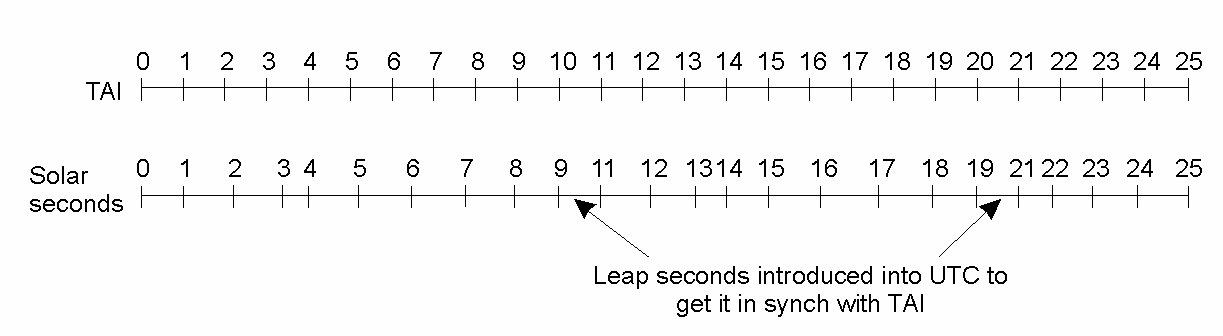
\includegraphics[scale=0.4]{img/tai.png}
\caption{Paragone tra secondi TAI e secondi solari}\label{fig:tai}
\end{figure}
\subsubsection{Global positioning system}
Come passo per arrivare alla vera sincronizzazione dei clock consideriamo un problema che la riguarda, vale a dire la determinazione della posizione geografica di una persona o di un oggetto sulla terra. Questo problema è risolto mediante l'utilizzo del \textbf{global position system} o \textbf{GPS}. Il GPS è un sistema distribuito basato su un sistema di 29 satelliti in orbita a 20.000 km di altezza. Ogni satellite possiede fino a quattro orologi atomici, regolarmente calibrati da speciali stazioni sulla terra. \\
Ogni satellite diffonde continuamente la sua posizione e contrassegna ogni messaggio con il suo \emph{timestamp} locale.
Questa diffusione consente ad ogni soggetto sulla terra di calcolare con accuratezza la sua posizione.\\
Partiamo dal caso bidimensionale mostrato in \figurename\,\ref{fig:gps} in cui sono segnati due satelliti e le circonferenze che rappresentano i punti alla stessa distanza rispetto al satellite. L'asse $y$ rappresenta l'altezza mentre l'asse $x$ rappresenta una linea retta sulla terra a livello del mare. Ignorando il punto più in alto vediamo come l'intersezione delle circonferenze porti ad un punto univoco. Il principio dell'intersezione delle circonferenze può essere esteso a 3 satelliti per conoscere longitudine latitudine e altitudine.
\begin{figure}
\centering
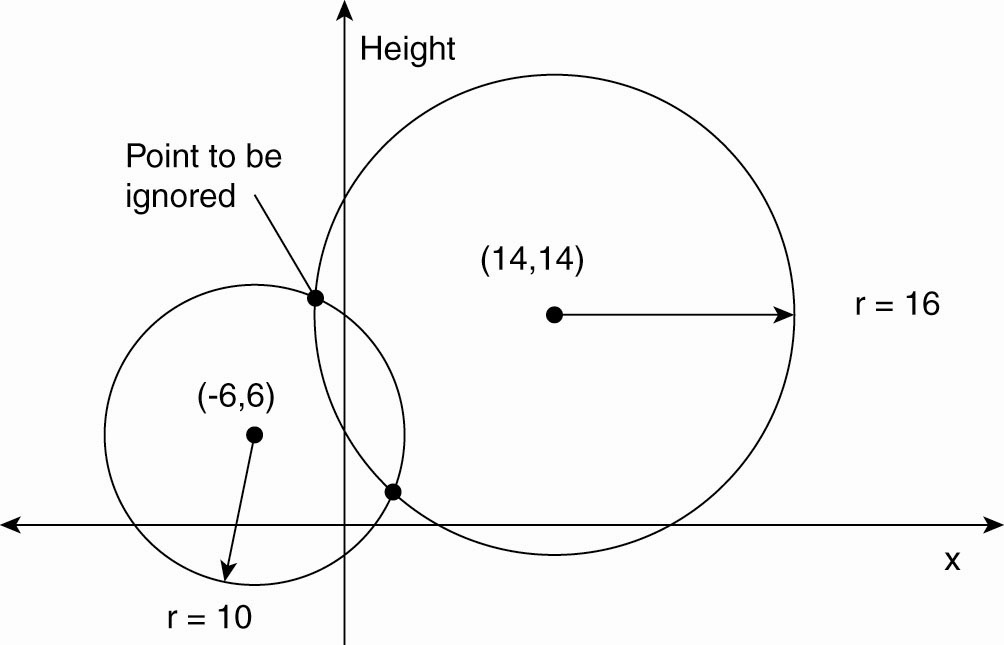
\includegraphics[scale=0.4]{img/gps.png}
\caption{Calcolo della posizione in uno spazio bidimensionale}\label{fig:gps}
\end{figure}
Ora supponiamo che gli orologi dei satelliti non siano perfettamente sincronizzati. Dobbiamo tener conto inoltre anche di due caratteristiche:
\begin{itemize}
\item ci vuole un certo tempo perchè i dati sulla posizione del satellite raggiungano il soggetto;
\item l'orologio del soggetto in genere non è sincronizzato con quello del satellite.
\end{itemize}
Supponiamo che il \emph{timestamp} del satellite sia assolutamente accurato. Definiamo ora $\Delta_r$ come la deviazione dell'orologio del soggetto rispetto al tempo reale, $T_i$ è il timestamp del messaggio ricevuto dal satellite $i$ e il tempo di trasferimento di tale messaggio è indicato come $\Delta_i$ che viene misurato dal soggetto ed è dato dal tempo di trasferimento reale e dalla sua deviazione. Abbiamo quindi che:
$$T_{now} = T_r - \Delta_r$$
$$\Delta_i = T_r - T_i$$
$$\Delta_i = (T_{now} - T_i)+\Delta_r$$
Dato che i segnali viaggiano alla velocità della luce $c$ la distanza del satellite è data da $c\Delta_i$:
$$d_i = c \Delta_i = c \times (T_now - T_i) + c \times \Delta_r$$
La distanza calcolata dalla prima parte dell'espressione può essere rappresentata come 
$$\sqrt{(x_i-x_r)^2+(y_i-y_r)^2+ (z_i-z_r)^2}$$
Se prendiamo in considerazione quattro satelliti otteniamo un sistema di quattro  equazioni e quattro incognite ($x_r,y_r,z_r,\Delta_r$)
\subsubsection{Algoritmi di sincronizzazione dei clock}
Se una macchina ha un ricevitore WWV l'obiettivo è quello di mantenere le altre macchine il più possibile allineate a questa. Sono stati proposti diversi algoritmi che tuttavia si basano sullo stesso sistema. Si suppone che ogni macchina abbia un timer che solleva un interrupt $H$ volte al secondo. Quando il timer scade, il gestore dell'interrupt aggiunge 1 all'orologio software. Chiamando $C$ questo valore  e $t$ il valore dell'UTC in un determinato istante avremo che in un mono perfetto $C_p(t) = t$ dove il pedice $p$ indica una determinata macchina. Definito inoltre $C'_p(t) = dC/dt$ la frequenza del clock di $p$ al tempo $t$ il \textbf{disallineamento} del clock viene definito come $C'_p - 1$ e denota qual'è lo scostamento della frequenza dal clock perfetto. L'\textbf{offset} relativo ad un determinato istante $t$ è dato da  $C_p(t)-t$.
\paragraph{Algoritmo Cristian}
Un approccio comune a molti protocolli è quello di lasciare che i client contattino un \emph{time server}. Quest'ultimo può fornire la data e l'ora attuali con precisione. Il problema principale di questo algoritmo è che il tempo di trasferimento dei messaggi rende obsolete data e ora. Il trucco è di trovare una stima valida per questo tempo di trasferimento.\\
Considerando la \figurename\,\ref{fig:cristian}.  In questo caso $A$ invia una richiesta a $B$ e la contrassegna con il \emph{timestamp} $T_1$, $B$ a sua volta memorizza l'istante di ricezione $T_2$ e restituisce una risposta contrassegnata con il timestamp $T_3$ che oltre all'orario si porta dietro anche il valore di $T_2$. Infine $A$ memorizza l'istante di arrivo $T_4$; supponendo che il tempo di trasmissione da $A$ a $B$ sia pressoché uguale a quello da $B$ ad $A$ il che significa che $T_2 - T_1 \approx T_4 - T_3$ allora si può stimare l'offset relativo a $B$ come
$$\theta = T_3 - \frac{(T_2 - T_1)+(T_4 - T_3)}{2}= \frac{(T_2 - T_1)+(T_3 - T_4)}{2}$$
\begin{figure}
\centering
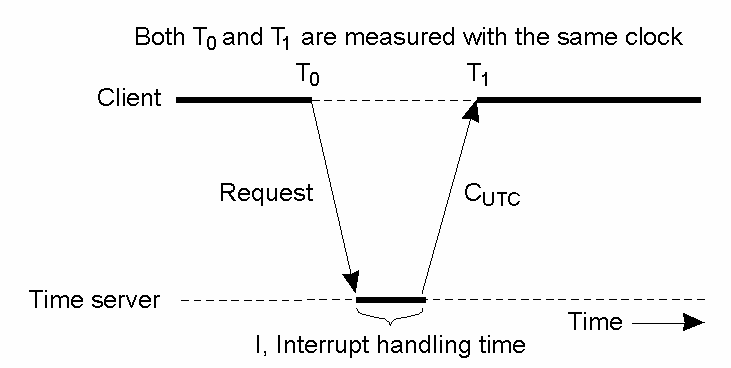
\includegraphics[scale=0.5]{img/cristian.png}
\caption{Esempio di scambio dei messaggi nell'algoritmo cristian}\label{fig:cristian}
\end{figure}
Se il clock di $A$ è veloce otterremo un $\theta<0$ questo significa che il clock di $A$ teoricamente dovrebbe tornare indietro. Questo però è impossibile in quanto provocherebbe potrebbe provocare parecchi problemi. Il cambiamento perciò deve essere introdotto gradualmente.\\
Nel \textbf{network time protocol} o NTP, che è un algoritmo basato su quello di Cristian si utilizzano otto stime dell'ora e si sceglie quello che ha un tempo medio di trasferimento minimo.
\paragraph{Algoritmo di Berkeley}
In molti algoritmi il \emph{time server} è passivo, sono le altre macchine che periodicamente chiedono l'ora. Tutto ciò che esso fa è rispondere alle richieste. In UNIX Berkley si esegue l'approccio esattamente opposto. In questo caso il \emph{time server} è attivo e di tanto in tanto richiede data e ora a tutte le macchine. In base alla risposta esso calcola un tempo medio e lo comunica alle altre macchine le quali si devono adeguare. Questo metodo è adatto per quelle macchine che non hanno un ricevitore WWV ma in questo caso la data e l'ora dei \emph{time daemon} devono essere impostate manualmente dall'operatore. Un esempio di questo algoritmo è mostrato in \figurename\,\ref{fig:berkley}
\begin{figure}
\centering
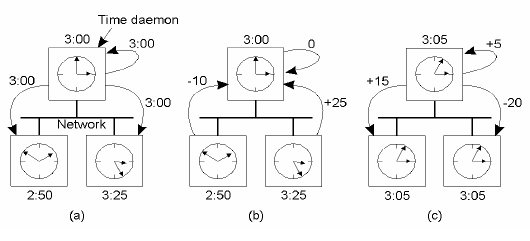
\includegraphics[scale=0.5]{img/berkley.png}
\caption{Esempio di algoritmo di berkley in (a) il server richiede l'ora, calcola una media (b) e invia le correzzioni (c)}\label{fig:berkley}
\end{figure}
In questo sistema non è essenziale che il tempo corrisponda a quello reale, se la rete è chiusa ovvero non ci sono comunicazioni con altri computer su internet non vi sarebbe alcun danno.
\subsection{Orologi logici}
Fino ad ora abbiamo supposto che la sincronizzazione sia naturalmente correlata con il tempo reale. Tuttavia abbiamo anche notato che la cosa importante è che i nodi concordino sulla data e sull'ora attuali senza che esse corrispondano a quelli reali (Berkley).\\
Riprendiamo ora il caso del \emph{make}, l'importante è che i nodi concordino sul fatto che il file \emph{input.o} sia diventato obsoleto a causa di una nuova versione del file \emph{input.c}. In questo caso l'unica cosa importante è tener traccia dei reciproci eventi. Per questi algoritmi si parla di \textbf{orologi logici}.
\subsubsection{Clock scalari}
Per sincronizzare gli orologi logici, Lamport ha definito una \textbf{relazione di precedenza} (\emph{happens-before}) che viene indicata da $a\rightarrow b$ e si legge come "\emph{a} precede \emph{b}" e sta ad indicare che tutti i processi concordano sul fatto che prima accade l'evento $a$ e poi accade l'evento $b$.
Esistono alcune situazioni in cui la relazione di precedenza può essere osservata:
\begin{enumerate}
\item Se $a$ e $b$ sono eventi dello stesso processo e $a$ precede $b$ allora $a \rightarrow b$ è vera.
\item Se $a$ è l'evento invio di un messaggio da parte di un processo e $b$ è l'evento di ricezione del messaggio da parte di un altro processo, allora $a \rightarrow b$ è di nuovo vera. Infatti è impossibile che un messaggio sia ricevuto prima di essere inviato.
\end{enumerate}
La relazione di precedenza è transitiva, per cui se $a\rightarrow b$ e $b \rightarrow c$ allora $a \rightarrow c$. Se $x$ e $y$ accadono in processi differenti che non si scambiano messaggi allora $x \rightarrow y$ non è vera ma non lo è nemmeno il suo opposto $y \rightarrow x$. In questi casi si dice che questi eventi sono \textbf{concorrenti} il che significa che non si può dire nulla su quanto accade.
\subsubsection{Clock vettoriali}
\subsection{Mutua esclusione}
\subsubsection{Panoramica}
\subsubsection{Un algoritmo centralizzato}
\subsubsection{Un algoritmo decentralizzato}
\subsubsection{Un algoritmo distribuito}
\subsubsection{Un algoritmo token ring}
\subsubsection{Confronto tra algoritmi}
\subsection{Algoritmi di elezione}
\subsubsection{Algoritmo di elezione tradizionale}
\subsubsection{Algoritmo di elezione token ring}
\subsection{Collection global state}
\subsubsection{Termination detection}
\subsection{Transizioni distribuite}
\subsubsection{Individuazione di deadlock distribuiti}